
	\documentclass{article}
	\usepackage{amsmath,amssymb}
	\usepackage[inline]{enumitem}
	\usepackage{blindtext}
	\usepackage{booktabs}
	\usepackage{graphicx}
	\usepackage{xcolor}
	\usepackage[vmargin = 1.5in, top = 1in, bottom = 1.2in, letterpaper]{geometry}
	\usepackage{listings}
	\usepackage{courier}
	\usepackage{bm}
	\lstset{
	basicstyle = \small\tt,
	keywordstyle = \tt\color{blue},
	commentstyle = \it\color[cmyk]{1,0,1,0},
	stringstyle = \tt\color[RGB]{128,0,0},
	%frame = single,
	backgroundcolor = \color[RGB]{245,245,244},
	breaklines,
	extendedchars = false,
	xleftmargin = 2em,
	xrightmargin = 2em,
	aboveskip = 1em,
	tabsize = 4,
	showspaces = false
	}
	\begin{document}
	
	% \newfontfamily\courier{Courier New}

	
	\title{STAT 500 Homework 8}
	\author{Yifan Zhu}
	\maketitle
	
	\begin{enumerate}[leftmargin = 0 em, label = \arabic*., font = \bfseries]
	\item
	\begin{enumerate}
		\item \
\begin{center}
		\begin{tabular}{lllllll}
		\toprule
		Source&DF&Sum of Squares&Mean Square&F Value&Pr $>$ F\\
		\midrule
Ethanol&2&324.0000000&162.0000000&31.35&$<.0001$\\
AirFuelRatio&2&652.0000000&326.0000000&63.10&$<.0001$\\
Ethanol*AirFuelRatio&4&678.0000000&169.5000000&32.81&$<.0001$\\
Error&9&46.500000&5.166667&&\\
Corrected Total&17&1700.500000&&	\\
\bottomrule
		\end{tabular}
		\end{center}



\item The plot shows the differences in the pattern of means of 3 Ethanol levels over the air/fuel ratio levels. We can see the patterns of three air/ratio levels are different. Noticeable differences in these patterns indicate a significant interaction between the two factors.

\begin{center}
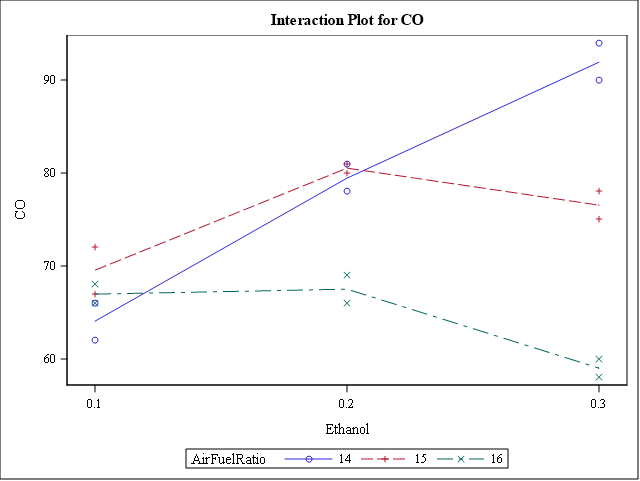
\includegraphics[width = 0.6\textwidth]{interaction.png}
\end{center}

\item From the table we can see both contrast have a p-value less than 0.05, thus there is a significant linear and quadratic effect.

\begin{tabular}{llllll}
\toprule
Contrast&DF&Contrast SS&Mean Square&F Value&Pr $>$ F\\
\midrule
E3-E1&1&243.0000000&243.0000000&47.03&$<.0001$\\
E2-(E1+E3)&1&81.0000000&81.0000000&15.68&$0.0033$\\
\bottomrule
\end{tabular}

\item From the table we can see both contrast have a p-value less than 0.05, thus there is a significant linear and quadratic effect.

\begin{tabular}{llllll}
\toprule
Contrast&DF&Contrast SS&Mean Square&F Value&Pr $>$ F\\
\midrule
AF3-AF1&1&588.0000000&588.0000000&113.81&$<.0001$\\
AF2-(AF1+AF3)&1&64.0000000&64.0000000&12.39&0.0065\\
\bottomrule
\end{tabular}


\item The Tukey HSD output from SAS indicates marginal means for Ethanol level 0.3 and 0.2 are not significantly different. Marginal mean for the Ethanol level 0.1 is significantly different from the other two with the lowest mean CO emission.
\begin{center}
	\begin{tabular}{llll}
	\toprule
Tukey Grouping&Mean&N&Ethanol\\
\midrule
A&75.833&6&0.3\\
A&75.833&6&0.2\\
B&66.833&6&0.1\\
\bottomrule
	\end{tabular}
\end{center}

\item The Tukey HSD output from SAS indicates marginal means for Air/Fuel Ratio level 14 and 15 are not significantly different. Marginal mean for the Air/Fuel Ratio level 16 is significantly different from the other two with the lowest mean CO emission.
\begin{center}
	\begin{tabular}{llll}
	\toprule
Tukey Grouping&Mean&N&Ethanol\\
\midrule
A&78.500&6&14\\
A&75.500&6&15\\
B&64.500&6&16\\
\bottomrule
	\end{tabular}
\end{center}


\item 
The points in the plot do not appear to have any patterns, so there is nothing of concern in this plot.
\begin{center}
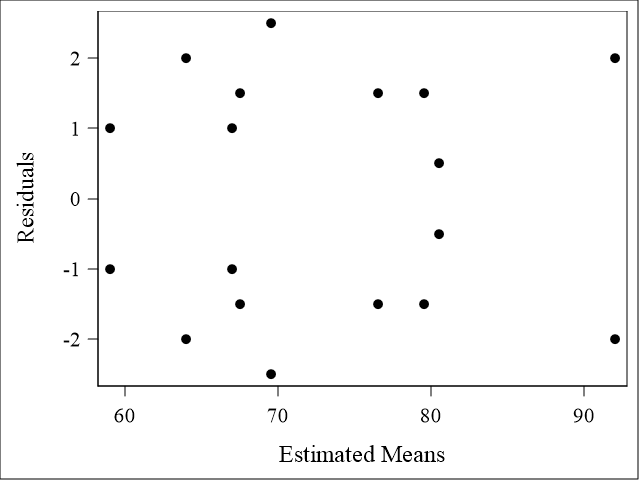
\includegraphics[width = 0.6\textwidth]{resem.png}
\end{center}


\item 
The variation in the residuals by Ethanol values and by Air/Fuel Ratio levels do not show any large differences. So there is nothing to concern of these two plots.

\begin{minipage}{0.5\textwidth}
	\begin{center}
		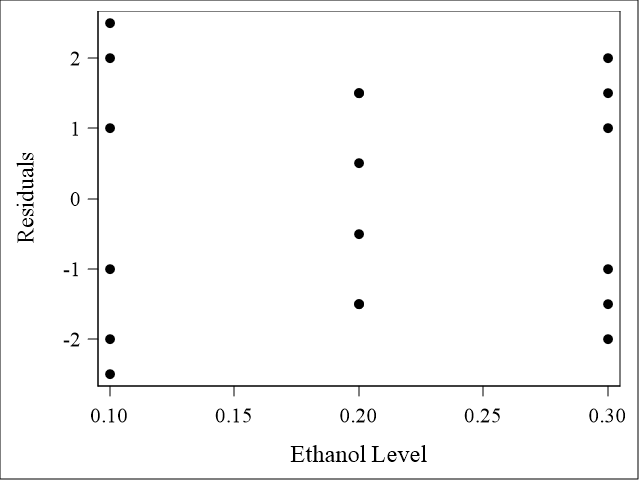
\includegraphics[width = 0.7\linewidth]{rese.png}
	\end{center}
\end{minipage}
\hspace{-4em}
\begin{minipage}{0.5\textwidth}
	\begin{center}
		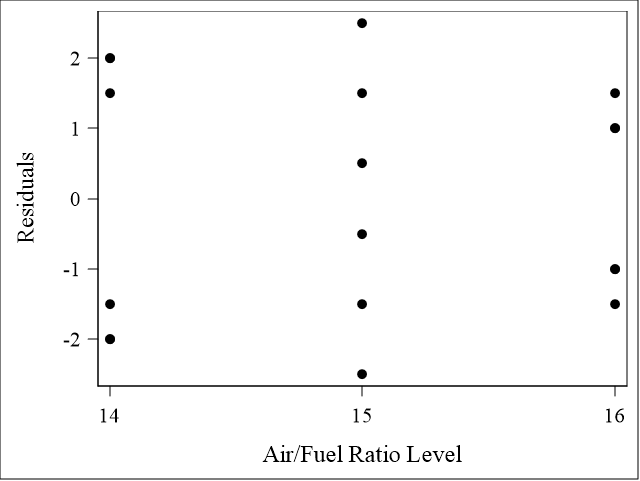
\includegraphics[width = 0.7\linewidth]{resaf.png}
	\end{center}
\end{minipage}


\newpage
\item 
The points fall in a straight line pattern, indicating the normal distribution assumption is met.

\begin{center}
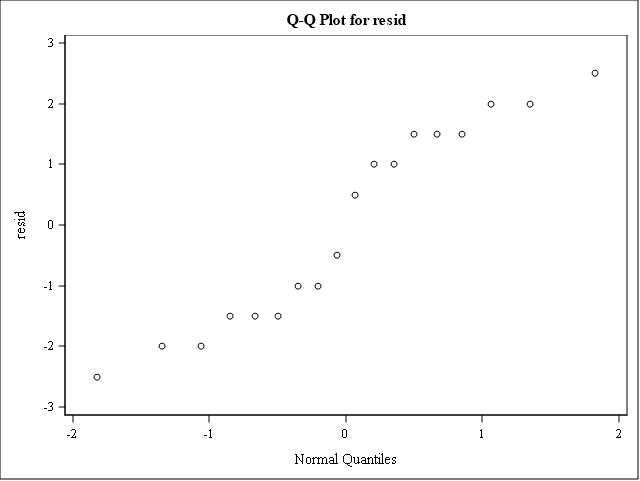
\includegraphics[width=0.6\textwidth]{qqnormal.png}
\end{center}
\end{enumerate}
\end{enumerate}
	
	\end{document}